\documentclass{standalone}



\usepackage{graphics}
\usepackage{color}
\usepackage{tikz}

\definecolor{blue}{RGB}{0, 114, 189}
\definecolor{red}{RGB}{212.5000,81.2500,   24.5000}
\definecolor{yellow}{RGB}{232.2500, 173.5000,   31.2500}
\definecolor{violet}{RGB}{123.5000,  46.0000, 139.0000}
\definecolor{green}{RGB}{116.5000, 168.5000,  47.0000}


\begin{document}
 \begin{figure}[h]
 \centering
  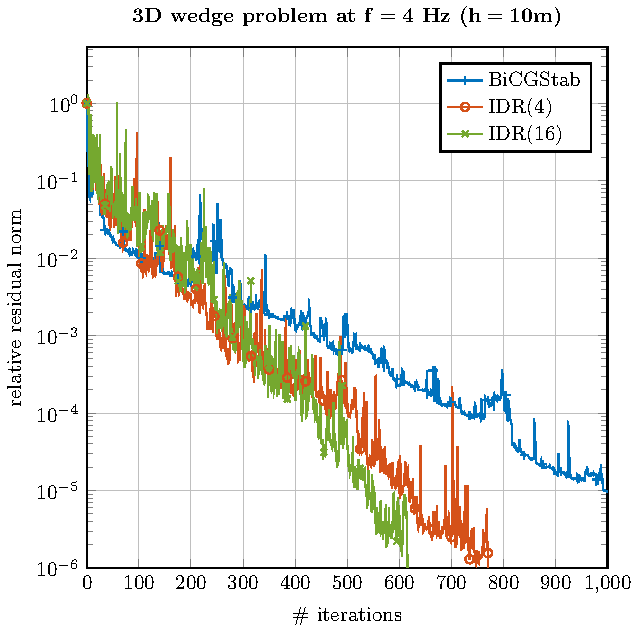
\includegraphics{wedge3d_f4_new2.pdf}
 \end{figure}
 
 \begin{tikzpicture}[overlay]
%   \draw[color=blue, thick] (-4.05,5.5) -- (-3.2,5.5) -- (-3.2,5.05) --cycle;
  \draw[color=blue, thick, dashed] (-4.85,5.5) -- (-3.15,5.5) -- (-3.15,4.6) --cycle;
  \node[color=blue, rotate=-28] at (-3.8,5.15) {\texttt{-3.5e-3}};
   
%   \draw[color=red, thick] (-8,5) -- (-8,4.2) -- (-7.15,4.2) --cycle;
%   \draw[color=red, thick] (-8,5) -- (-8,3.8) -- (-6.725,3.8) --cycle;
    \draw[color=red, thick, dashed] (-8,5) -- (-8,3.68) -- (-6.6,3.68) --cycle;
  \node[color=red, rotate=-44] at (-7.45,4.25) {\texttt{-6.2e-3}};
  
%   \draw[color=green, thick] (-5.9,2.55) -- (-5.9,1.5) -- (-5.05,1.5) --cycle;
  \draw[color=green, thick, dashed] (-5.9,3.075) -- (-5.9,1.5) -- (-4.625,1.5) --cycle;
  \node[color=green, rotate=-50] at (-5.4,2.2) {\texttt{-7.9e-3}};
 \end{tikzpicture}

 
\end{document}
